%\documentclass[a4paper,12pt]{report}
\documentclass[a4paper,12pt]{article}
%\documentclass[a4paper,12pt]{book}
\usepackage{polski}
\usepackage[polish]{babel}
\usepackage[utf8]{inputenc}
\usepackage[top=2.5cm, bottom=2.5cm, left=3cm, right=2.5cm]{geometry}
\usepackage{graphicx}
\usepackage{setspace}
\usepackage{ifthen}
%\usepackage[utf8]{inputenc}
\usepackage{a4wide}
\usepackage{fullpage}
\usepackage{verbatim}
\usepackage[usenames,dvipsnames]{color}
\usepackage{hyperref}
\usepackage{subfig}
\usepackage{listings}
\usepackage{mdwlist}
\usepackage{titlesec}
\usepackage{lipsum}
\usepackage{morefloats}

\begin{document}

\begin{figure}[!htb]
\centering 		
  \subfloat[Windows]{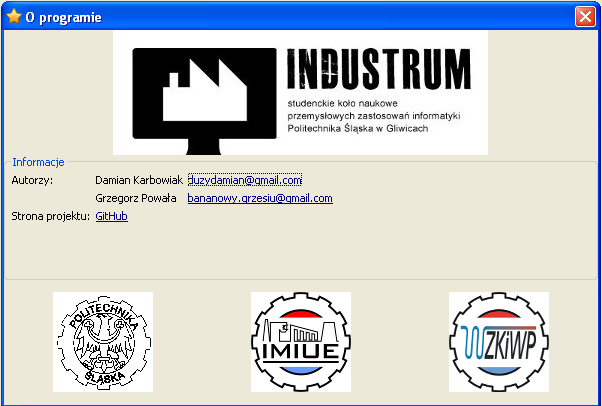
\includegraphics[width=0.49\textwidth]{images/aboutW}}    
  \hspace{1mm}
  \subfloat[Linux]{
\includegraphics[width=0.49\textwidth]{images/aboutL}}
\caption{Okno o programie} 	
\label{about}
\end{figure}

\begin{figure}[!htb]
\centering 		
  \subfloat[Windows]{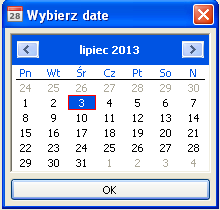
\includegraphics[width=0.25\textwidth]{images/calendarW}}    
  \hspace{2mm}
  \subfloat[Linux]{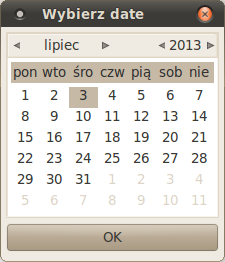
\includegraphics[width=0.25\textwidth]{images/calendarL}}
\caption{Okno wyboru daty} 	
\label{calendar}
\end{figure}

\begin{figure}[!htb]
\centering 		
  \subfloat[Windows]{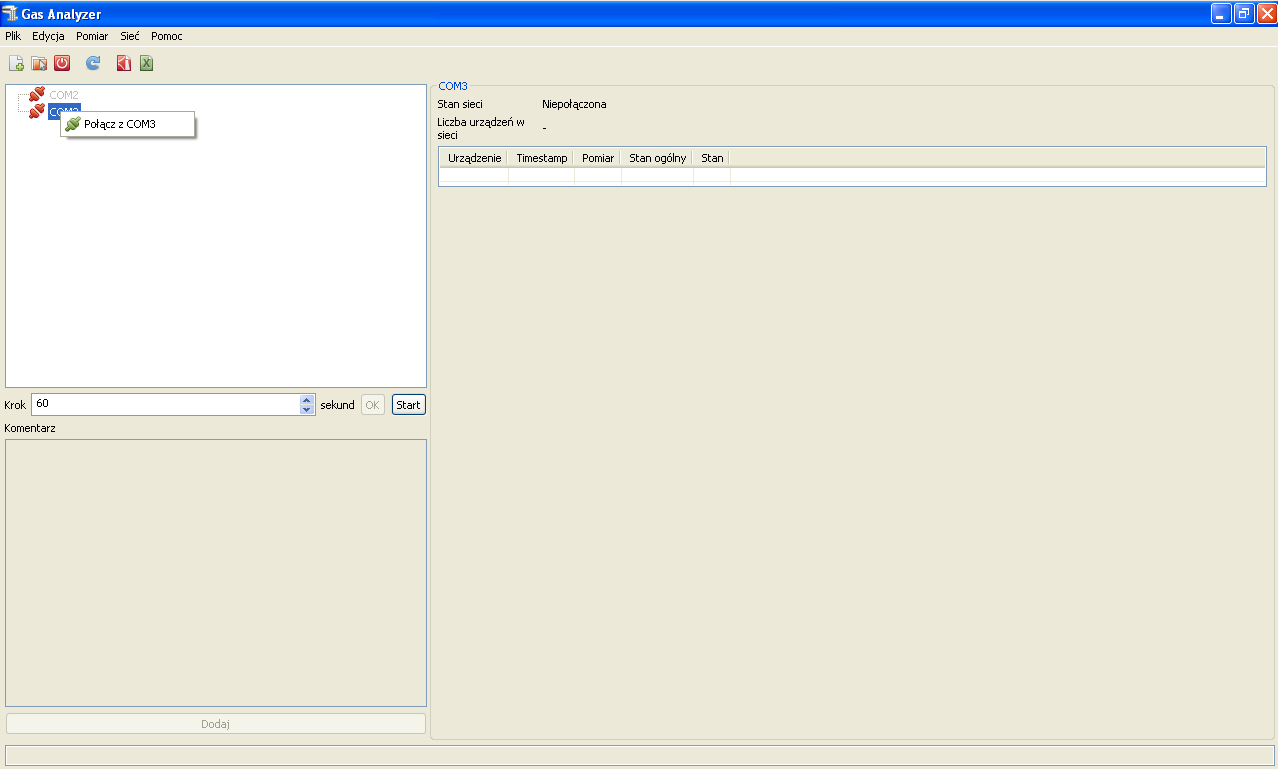
\includegraphics[width=0.49\textwidth]{images/connectW}}    
  \hspace{1mm}
  \subfloat[Linux]{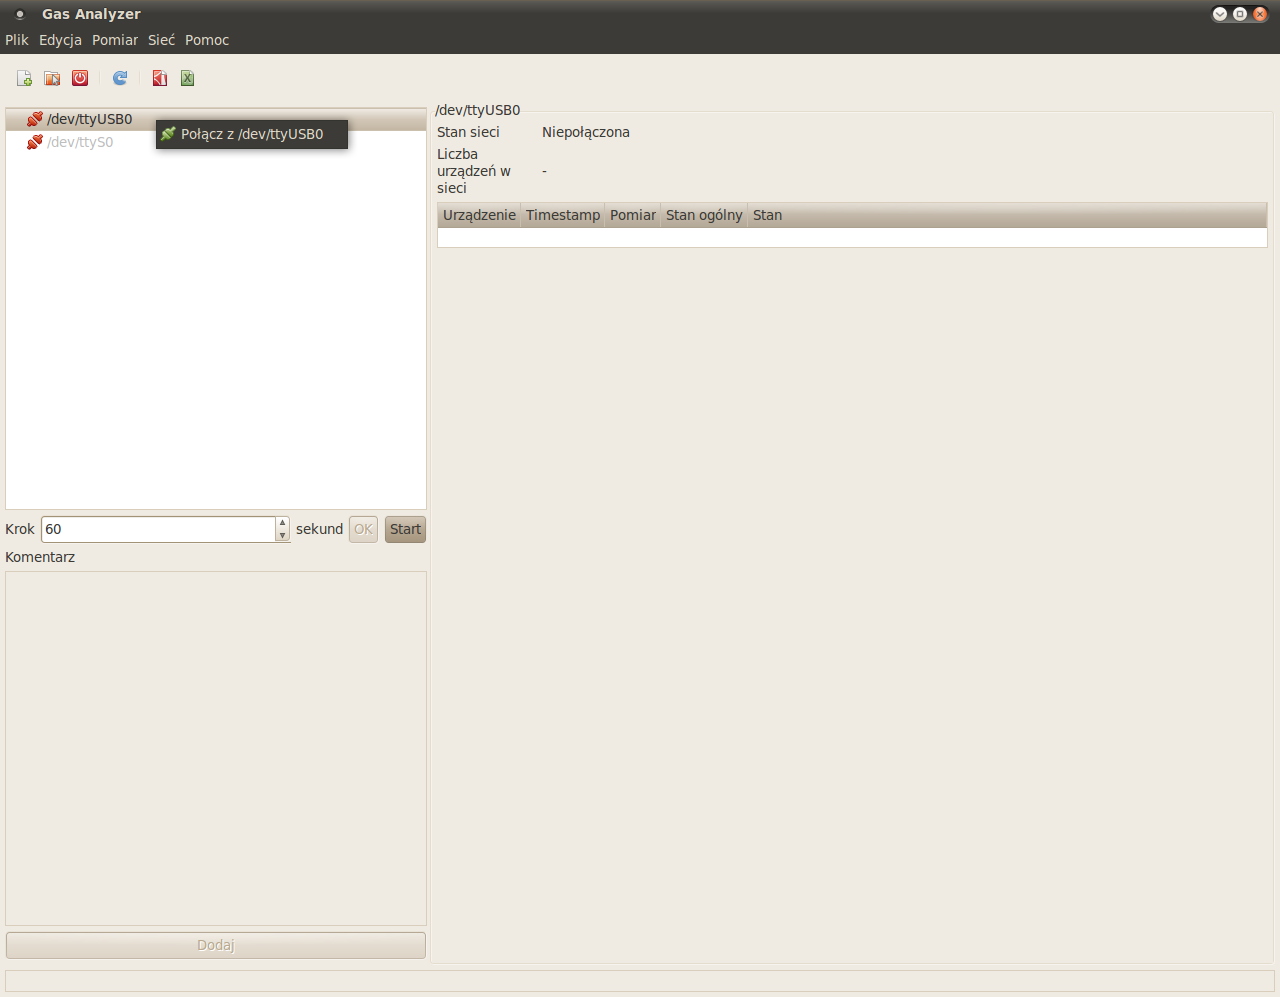
\includegraphics[width=0.49\textwidth]{images/connectL}}
\caption{Łączenie z siecią} 	
\label{connect}
\end{figure}

\begin{figure}[!htb]
\centering 		
  \subfloat[Windows]{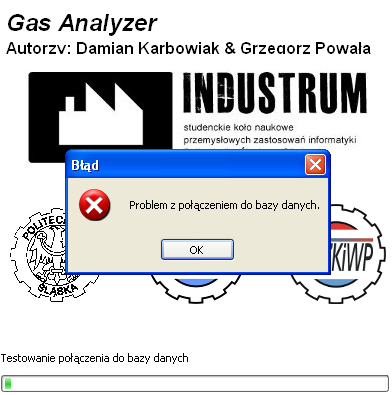
\includegraphics[width=0.35\textwidth]{images/dbErrorW}}    
  \hspace{1mm}
  \subfloat[Linux]{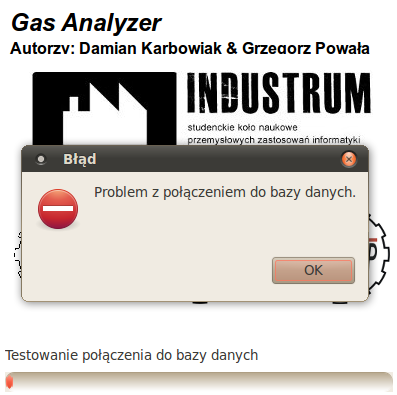
\includegraphics[width=0.35\textwidth]{images/dbErrorL}}
\caption{Komunikat o błędzie łączenia do bazy danych} 	
\label{dbError}
\end{figure}

\begin{figure}[!htb]
\centering 		
  \subfloat[Windows]{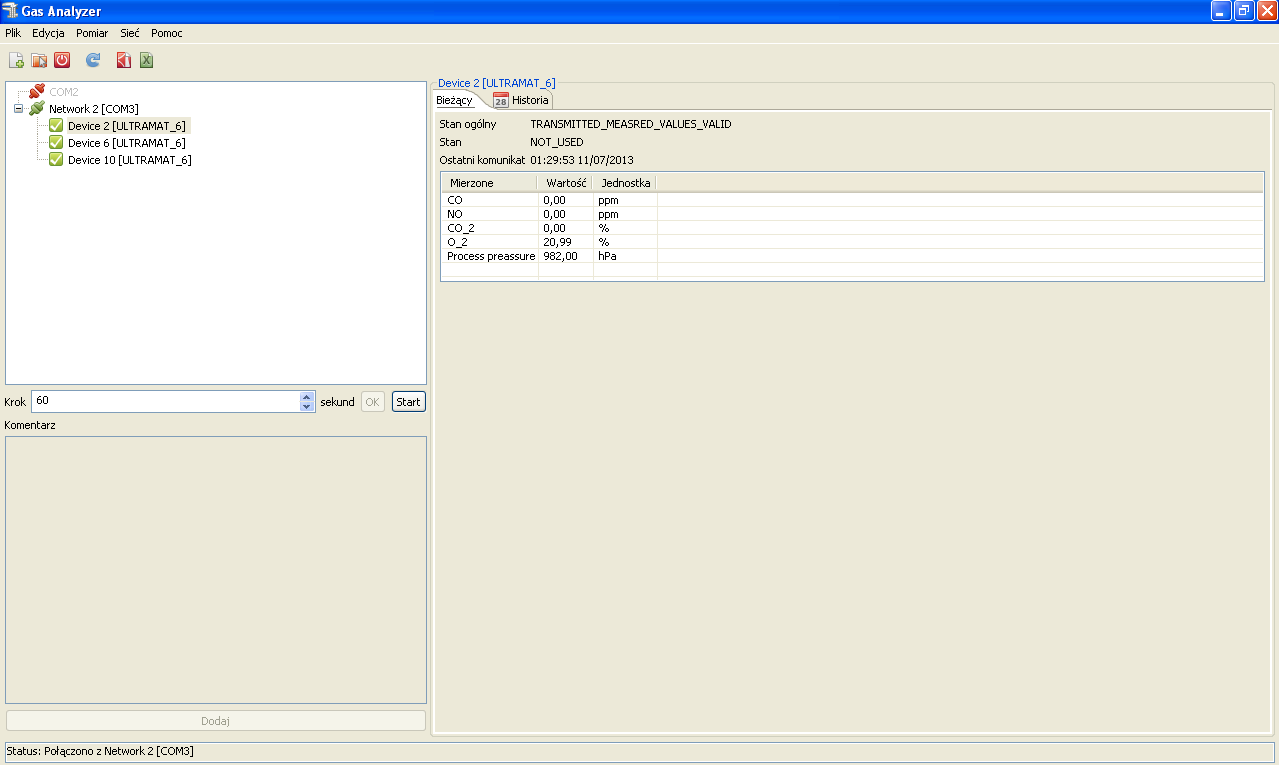
\includegraphics[width=0.49\textwidth]{images/detailDeviceW}}    
  \hspace{1mm}
  \subfloat[Linux]{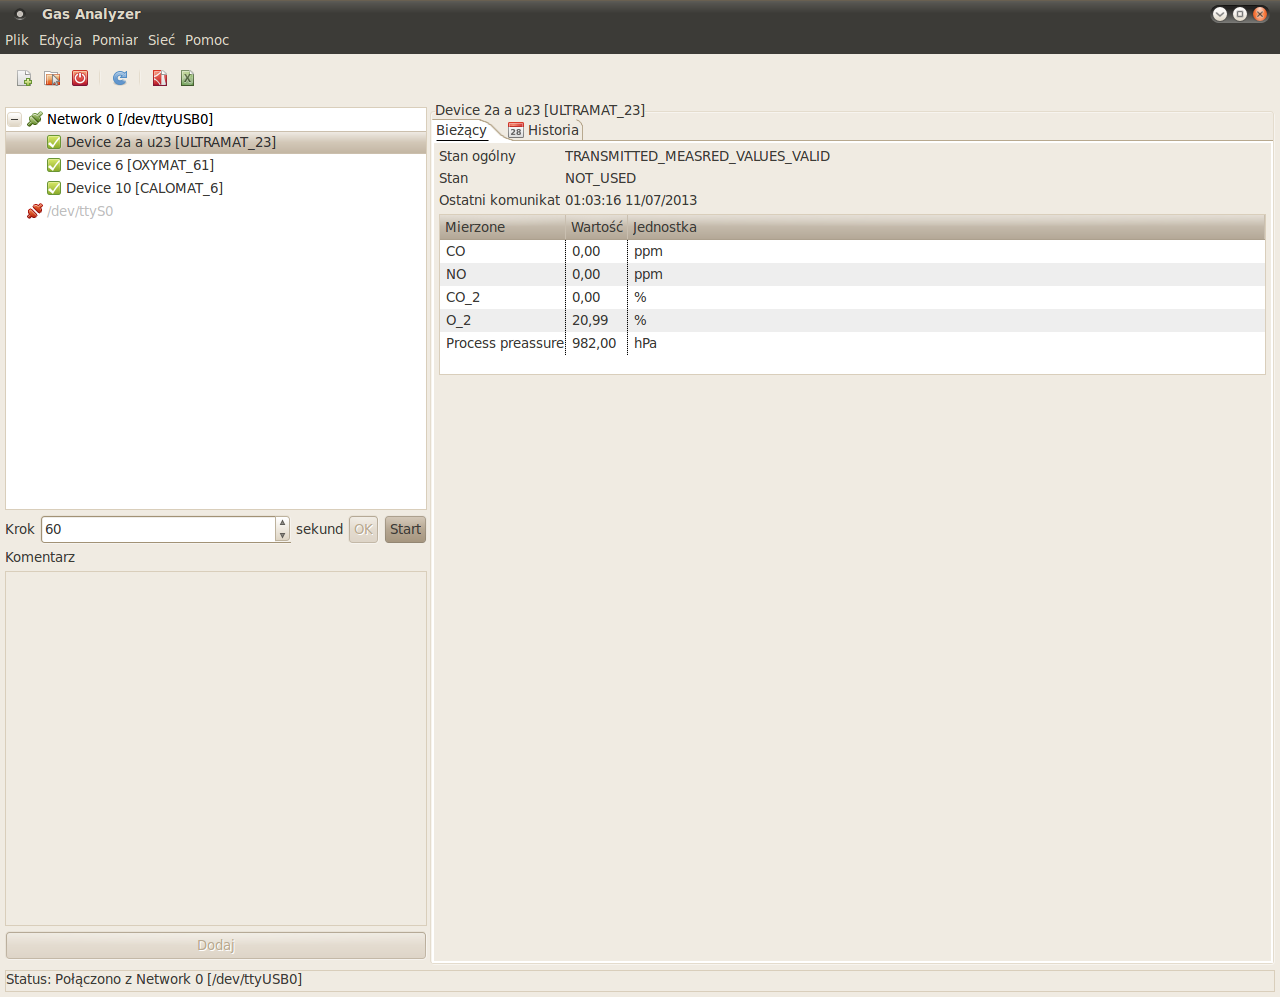
\includegraphics[width=0.49\textwidth]{images/detailDeviceL}}
\caption{Szczegółowy widok urządzenia} 	
\label{detailDevice}
\end{figure}

\begin{figure}[!htb]
\centering 		
  \subfloat[Windows]{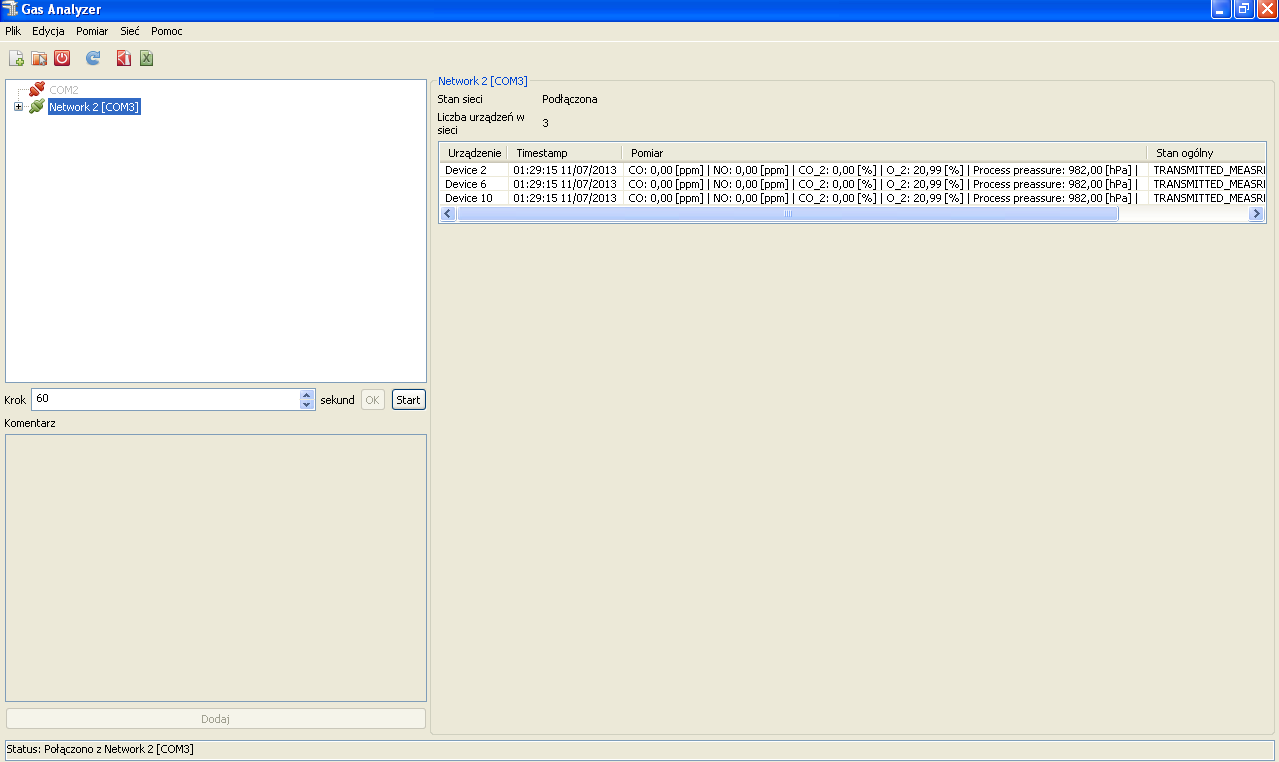
\includegraphics[width=0.49\textwidth]{images/detailNetworkW}}    
  \hspace{1mm}
  \subfloat[Linux]{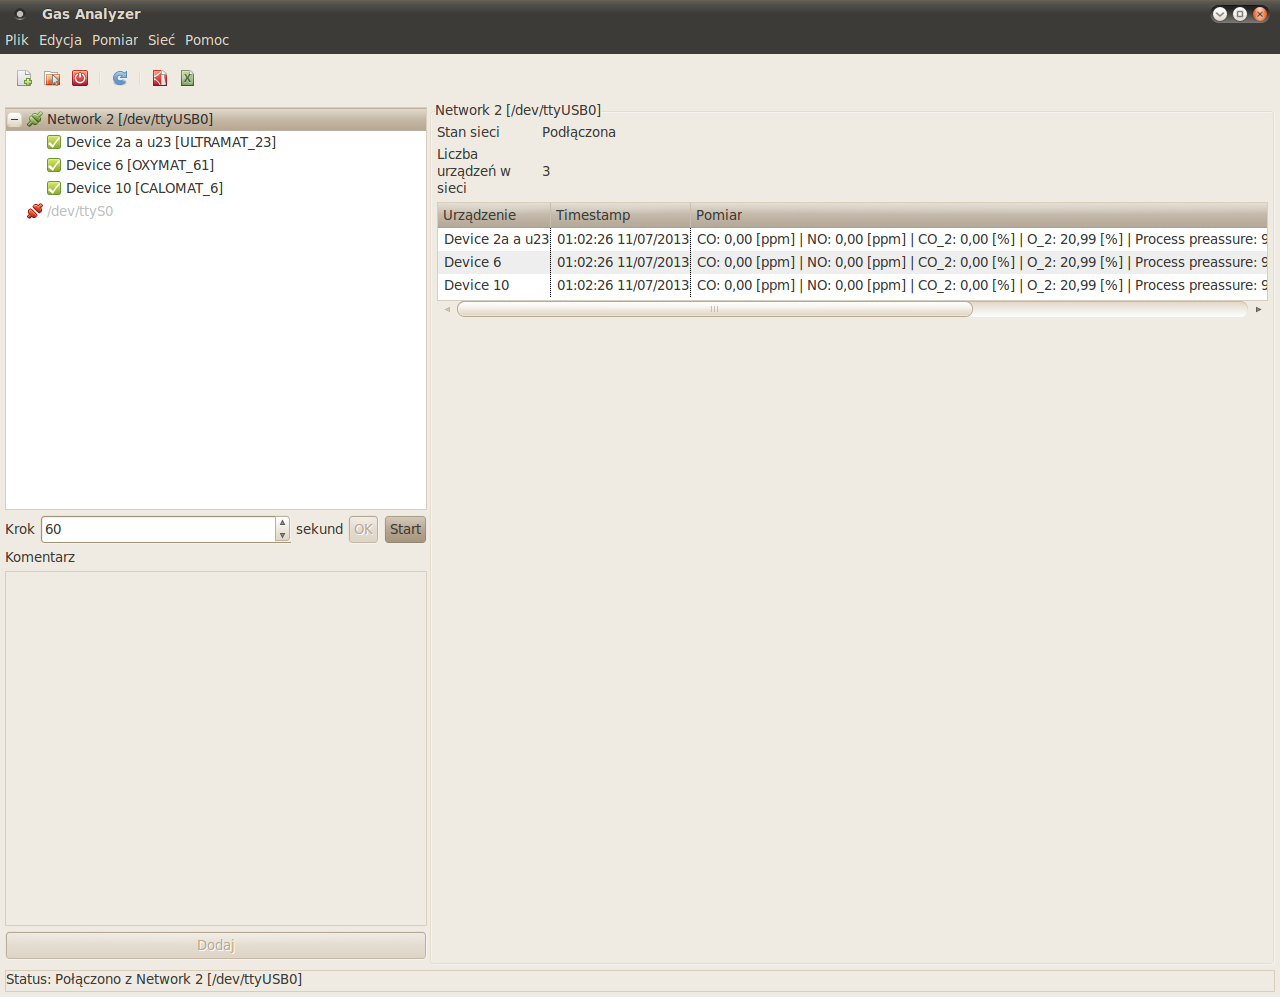
\includegraphics[width=0.49\textwidth]{images/detailNetworkL}}
\caption{Szczegółowy widok sieci} 	
\label{detailNetwork}
\end{figure}

\begin{figure}[!htb]
\centering 		
  \subfloat[Windows]{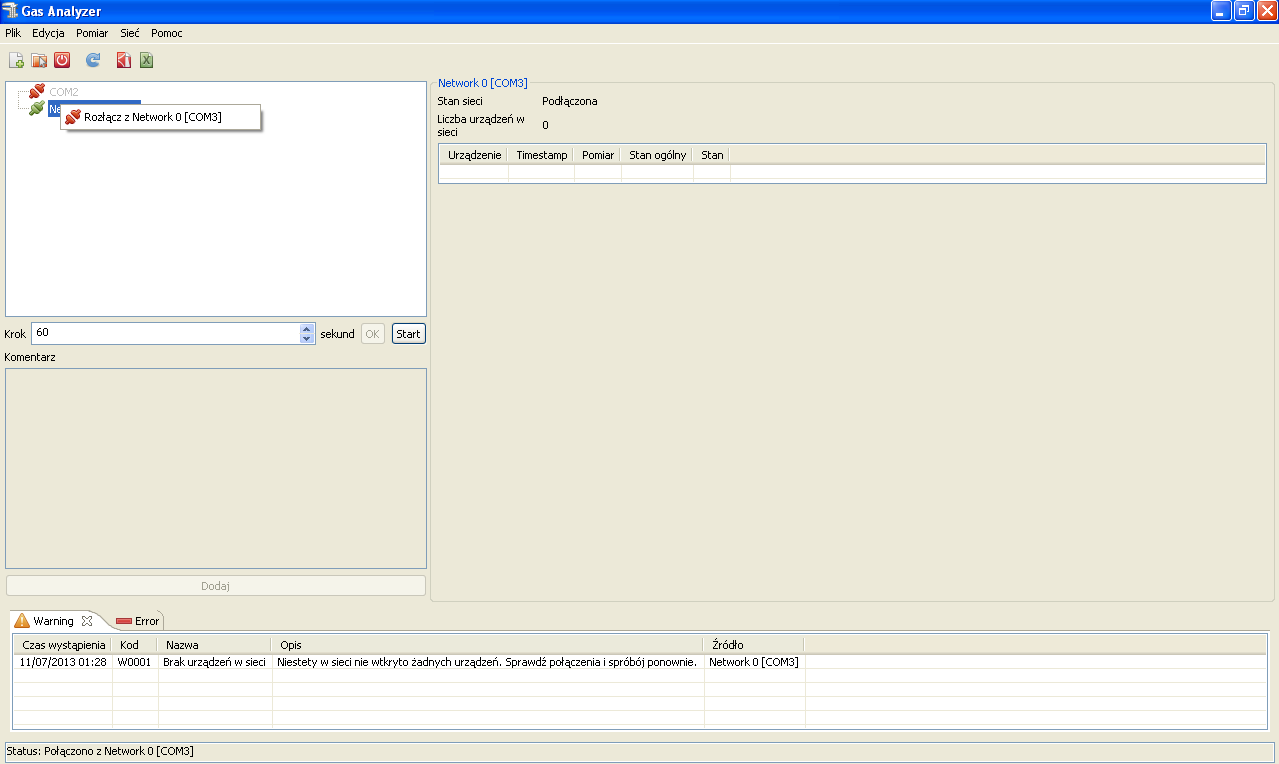
\includegraphics[width=0.49\textwidth]{images/disconnectW}}    
  \hspace{1mm}
  \subfloat[Linux]{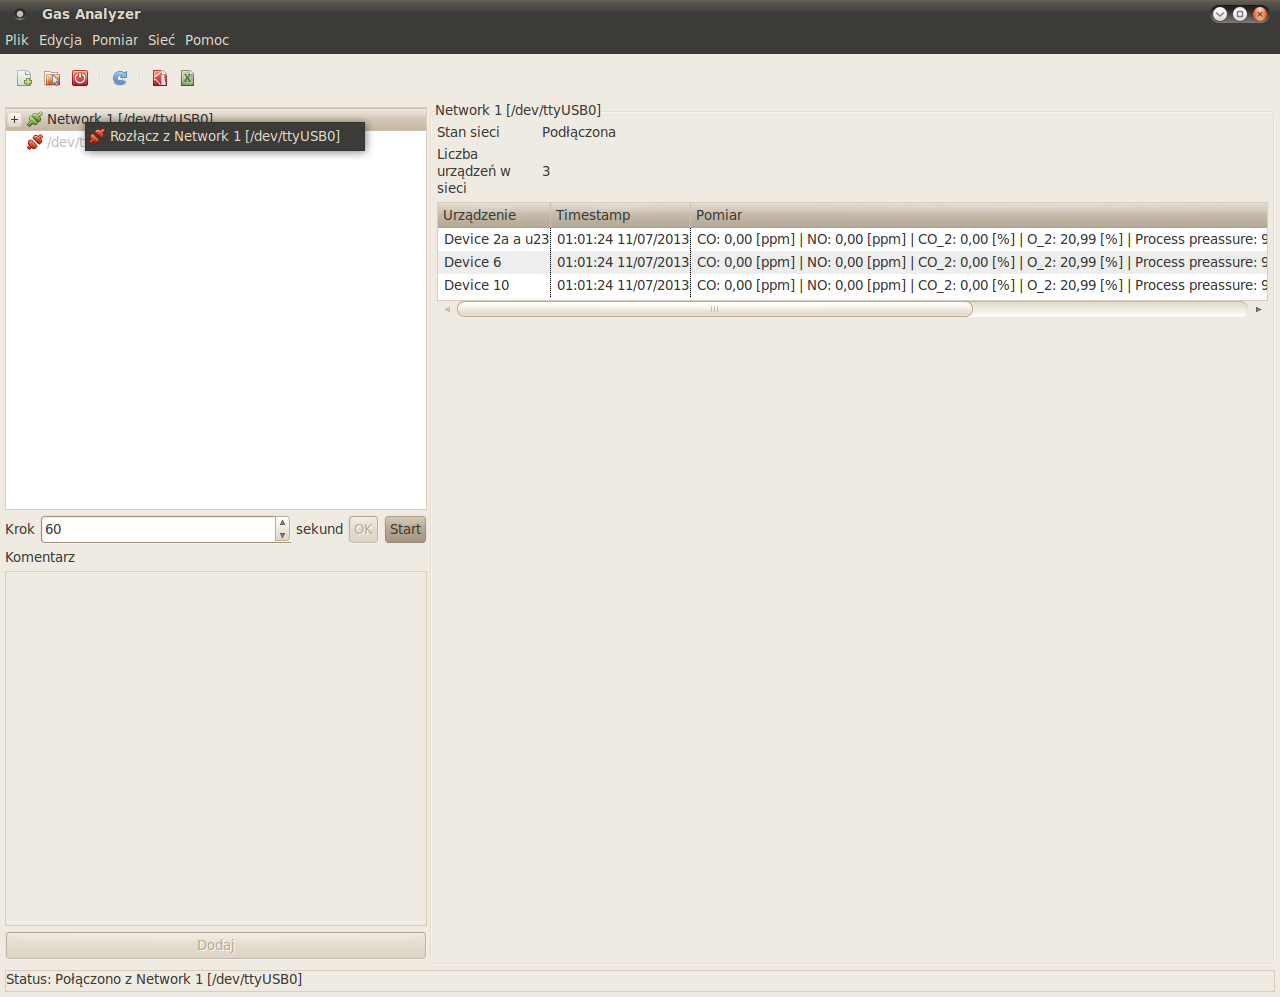
\includegraphics[width=0.49\textwidth]{images/disconnectL}}
\caption{Rozłączenie z siecią} 	
\label{disconnect}
\end{figure}

\begin{figure}[!htb]
\centering 		
  \subfloat[Windows]{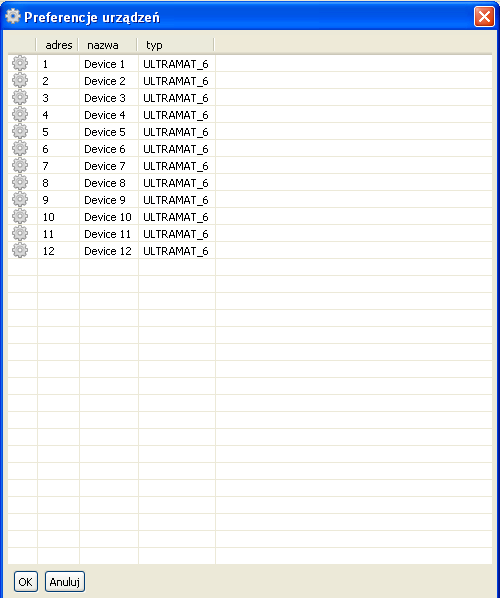
\includegraphics[width=0.45\textwidth]{images/editDeviceW}}    
  \hspace{1mm}
  \subfloat[Linux]{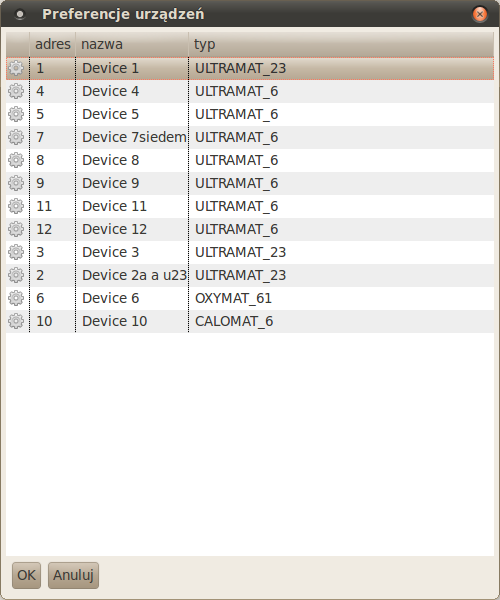
\includegraphics[width=0.45\textwidth]{images/editDeviceL}}
\caption{Okno edycji danych urzadzeń} 	
\label{editDevice}
\end{figure}

\begin{figure}[!htb]
\centering 		
  \subfloat[Windows]{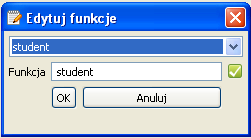
\includegraphics[width=0.35\textwidth]{images/editfFunctionW}}    
  \hspace{1mm}
  \subfloat[Linux]{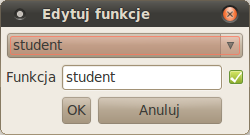
\includegraphics[width=0.35\textwidth]{images/editfFunctionL}}
\caption{Okno edycji funkcji} 	
\label{editFunction}
\end{figure}

\begin{figure}[!htb]
\centering 		
  \subfloat[Windows]{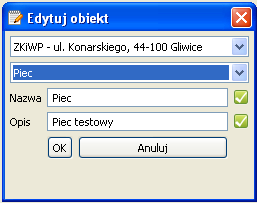
\includegraphics[width=0.35\textwidth]{images/editObjectW}}    
  \hspace{1mm}
  \subfloat[Linux]{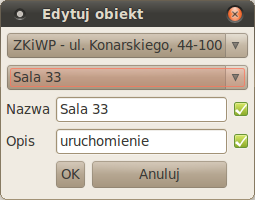
\includegraphics[width=0.35\textwidth]{images/editObjectL}}
\caption{Okno edycji obiektów} 	
\label{editObject}
\end{figure}

\begin{figure}[!htb]
\centering 		
  \subfloat[Windows]{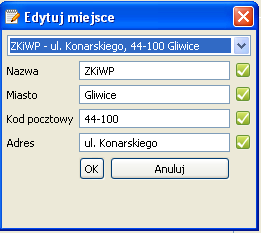
\includegraphics[width=0.35\textwidth]{images/editPlaceW}}    
  \hspace{1mm}
  \subfloat[Linux]{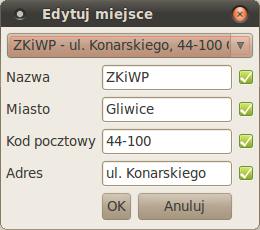
\includegraphics[width=0.35\textwidth]{images/editPlaceL}}
\caption{Okno edycji miejsc} 	
\label{editPlace}
\end{figure}

\begin{figure}[!htb]
\centering 		
  \subfloat[Windows]{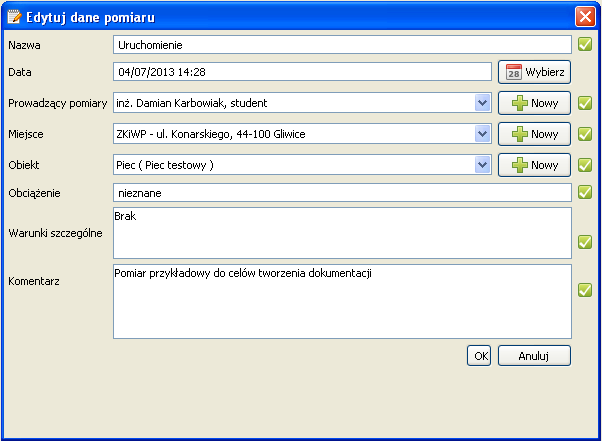
\includegraphics[width=0.49\textwidth]{images/editSurveyW}}    
  \hspace{1mm}
  \subfloat[Linux]{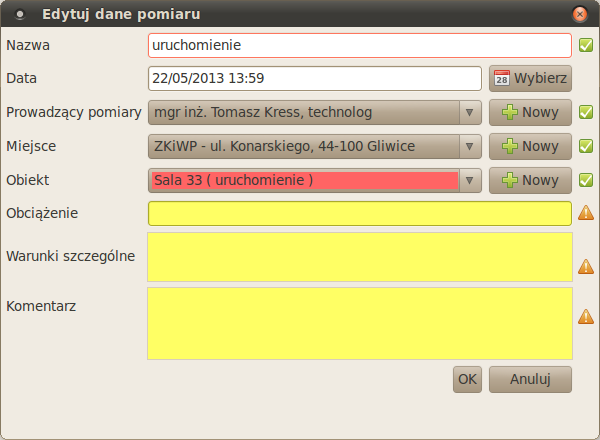
\includegraphics[width=0.49\textwidth]{images/editSurveyL}}
\caption{Okno edycji danych pomiaru} 	
\label{editSurvey}
\end{figure}

\begin{figure}[!htb]
\centering 		
  \subfloat[Windows]{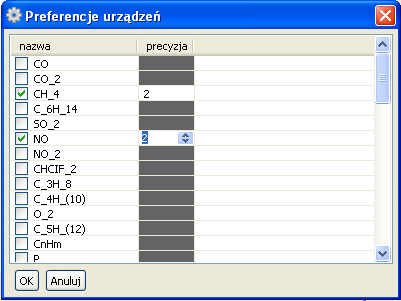
\includegraphics[width=0.45\textwidth]{images/editPrecisionW}}    
  \hspace{1mm}
  \subfloat[Linux]{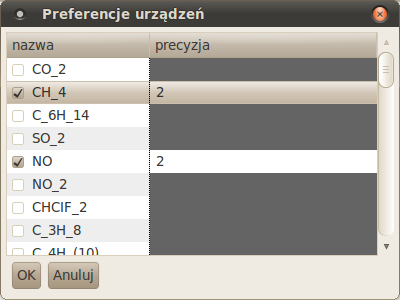
\includegraphics[width=0.45\textwidth]{images/editPrecisionL}}
\caption{Okno edycji precyzji pomiarowej} 	
\label{editPrecision}
\end{figure}

\begin{figure}[!htb]
\centering 		
  \subfloat[Windows]{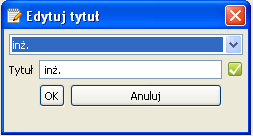
\includegraphics[width=0.35\textwidth]{images/editTitleW}}    
  \hspace{1mm}
  \subfloat[Linux]{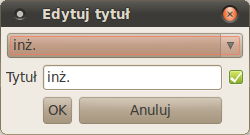
\includegraphics[width=0.35\textwidth]{images/editTitleL}}
\caption{Okno edycji tytułów naukowych} 	
\label{editTitle}
\end{figure}

\begin{figure}[!htb]
\centering 		
  \subfloat[Windows]{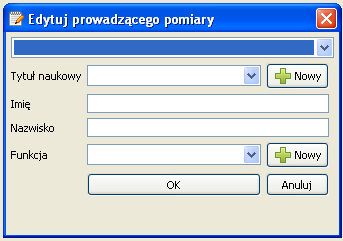
\includegraphics[width=0.35\textwidth]{images/editUserW}}    
  \hspace{1mm}
  \subfloat[Linux]{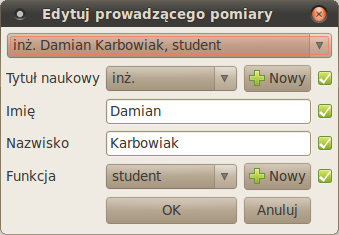
\includegraphics[width=0.35\textwidth]{images/editUserL}}
\caption{Okno edycji danych użytkownika} 	
\label{editUser}
\end{figure}

\begin{figure}[!htb]
\centering 		
  \subfloat[Windows]{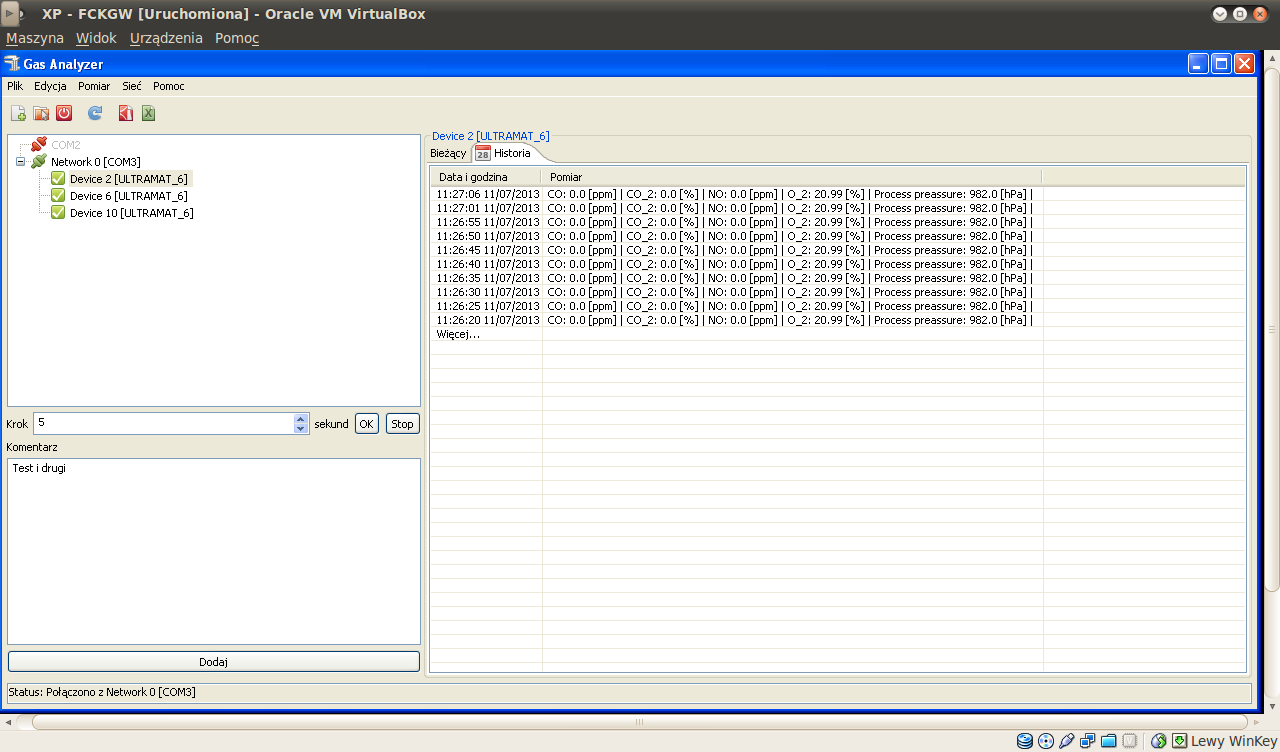
\includegraphics[width=0.49\textwidth]{images/historyLessW}}    
  \hspace{1mm}
  \subfloat[Linux]{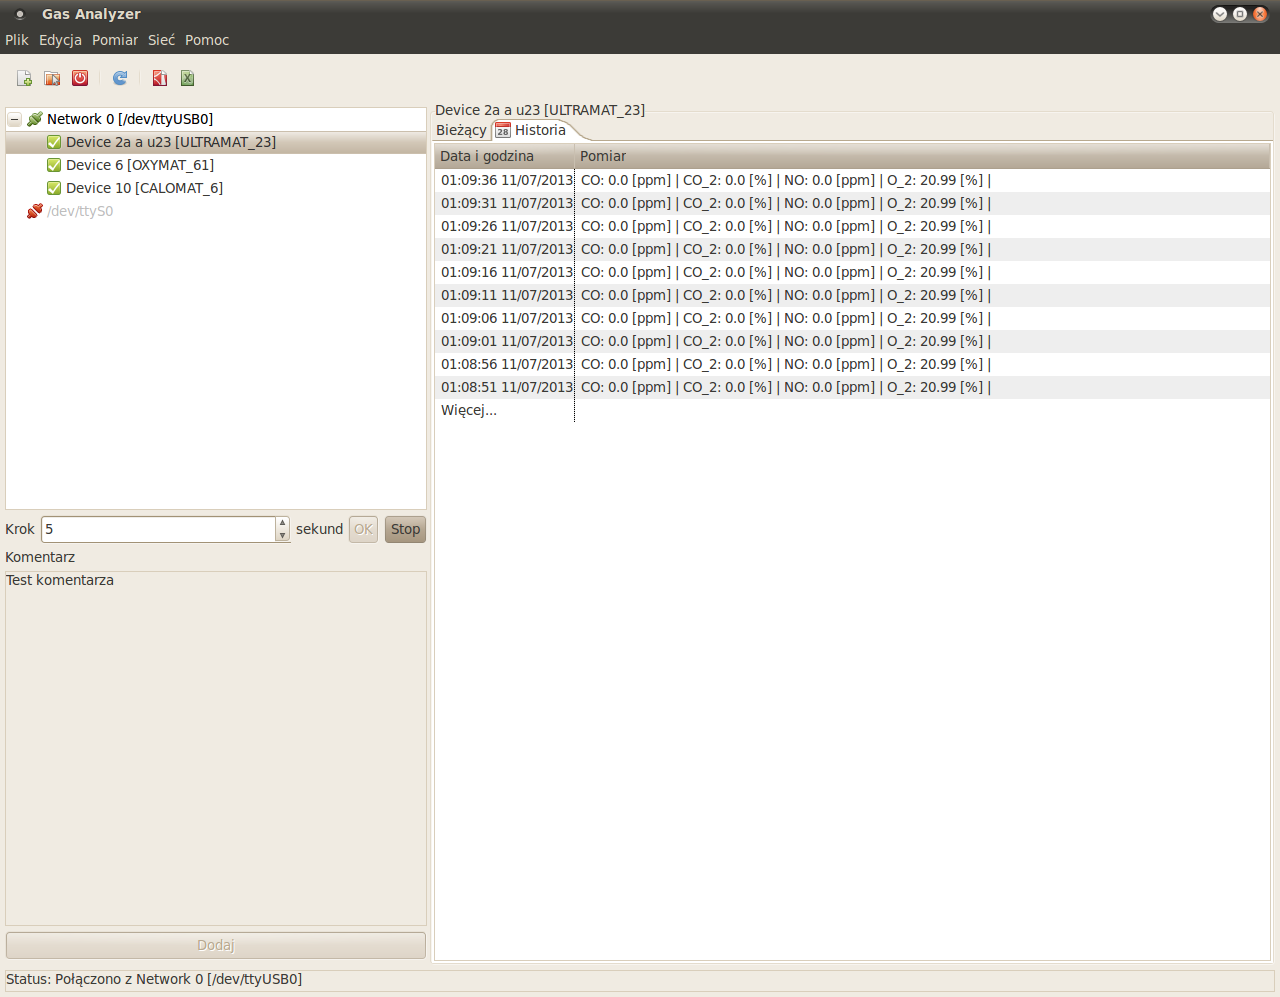
\includegraphics[width=0.49\textwidth]{images/historyLessL}}
\caption{Historia(mniej pomiarów)} 	
\label{historyLess}
\end{figure}

\begin{figure}[!htb]
\centering 		
  \subfloat[Windows]{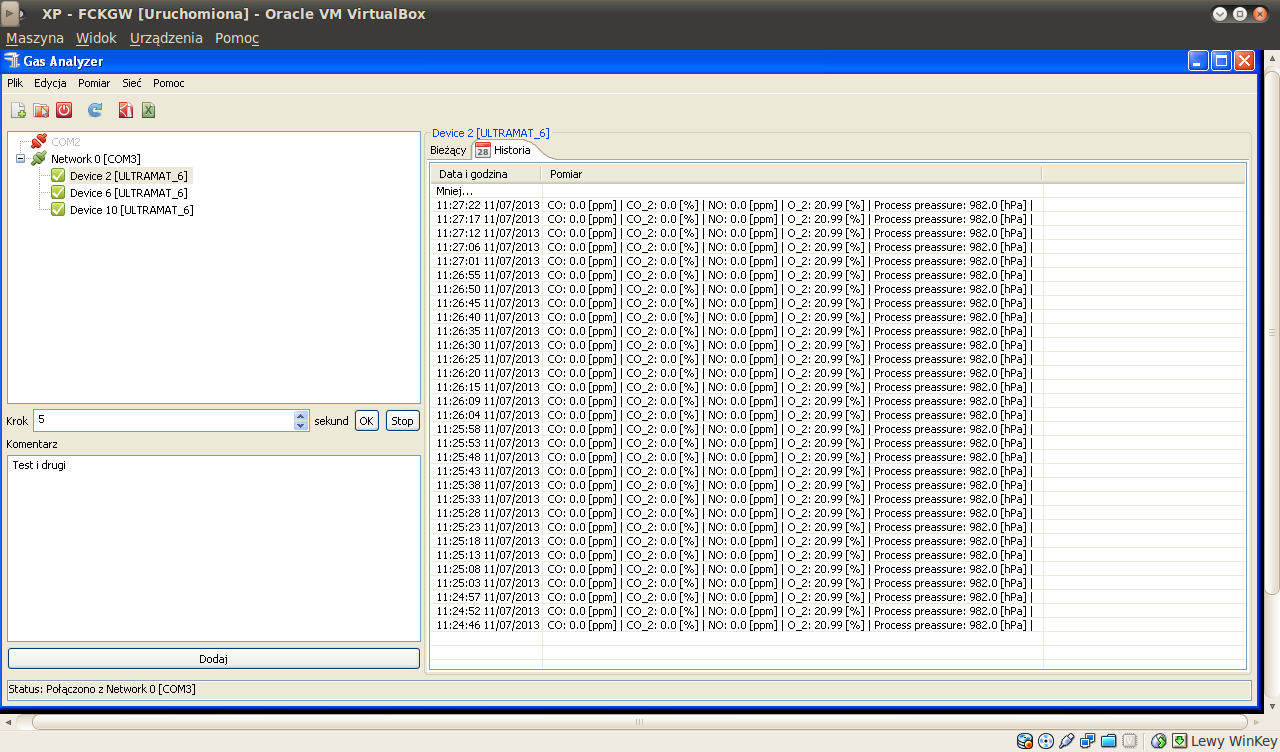
\includegraphics[width=0.49\textwidth]{images/historyMoreW}}    
  \hspace{1mm}
  \subfloat[Linux]{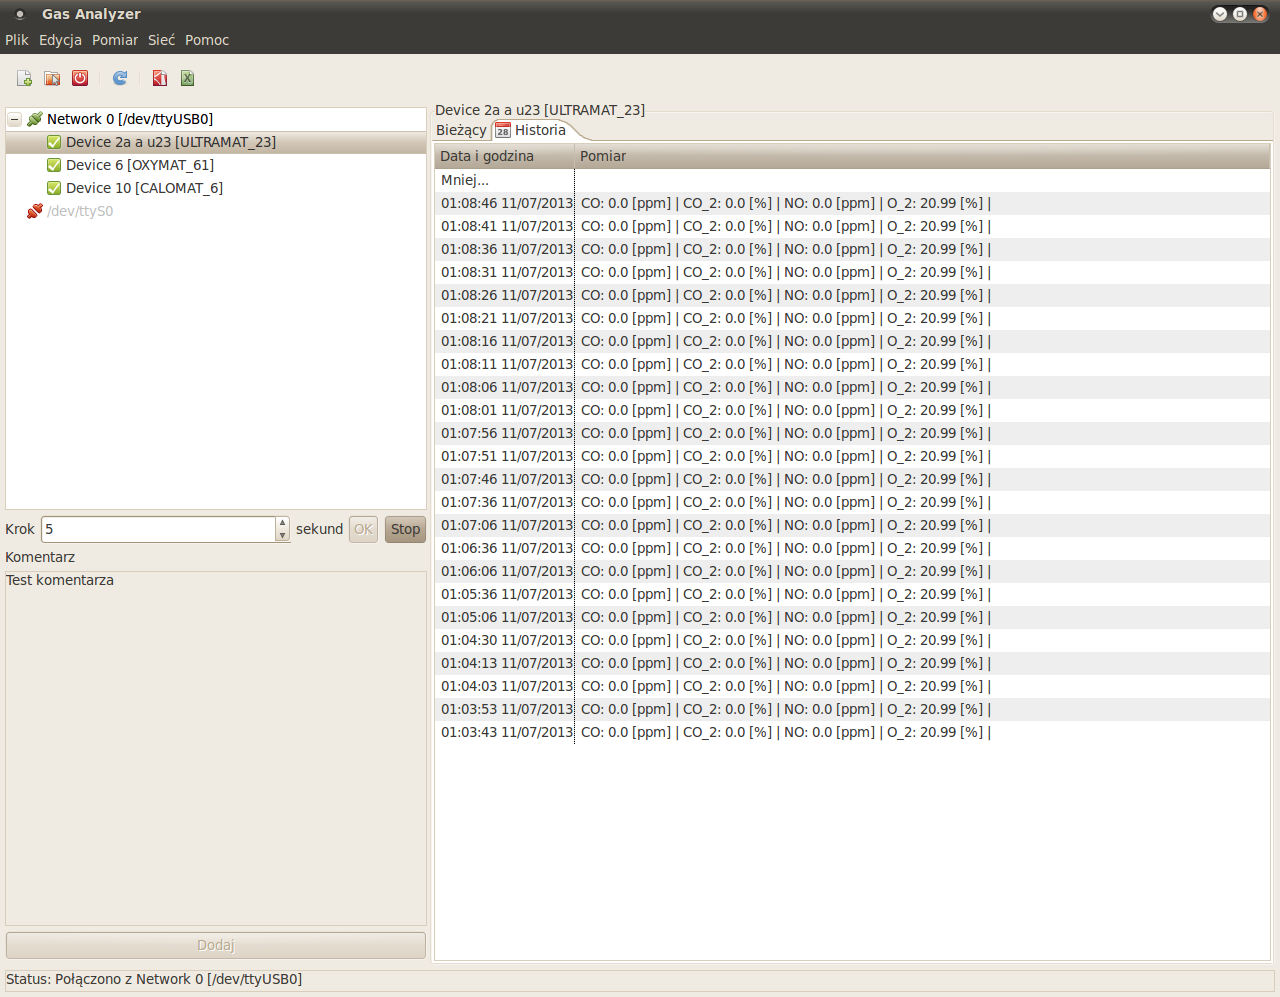
\includegraphics[width=0.49\textwidth]{images/historyMoreL}}
\caption{Historia(więcej pomiarów)} 	
\label{historyMore}
\end{figure}

\begin{figure}[!htb]
\centering 		
  \subfloat[Windows]{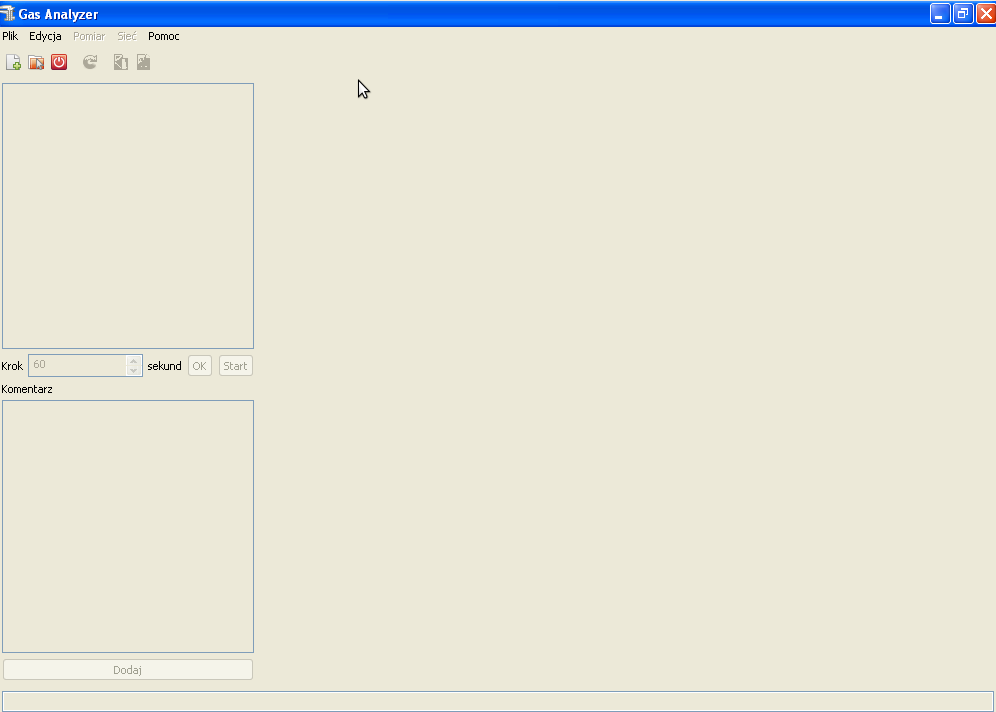
\includegraphics[width=0.49\textwidth]{images/mainW}}    
  \hspace{1mm}
  \subfloat[Linux]{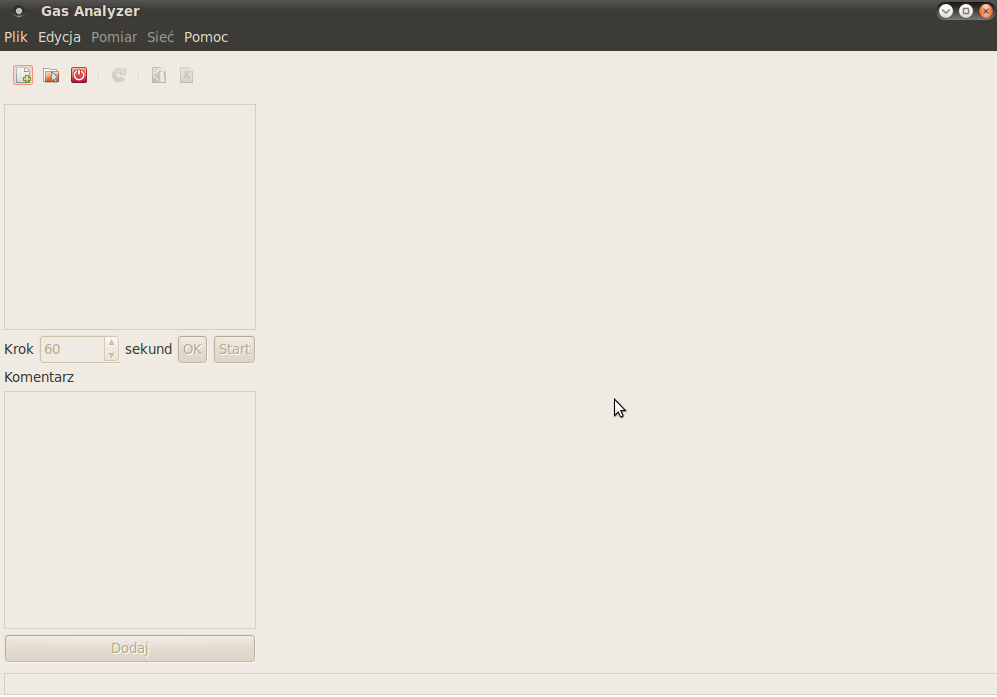
\includegraphics[width=0.49\textwidth]{images/mainL}}
\caption{Okno główne programu} 	
\label{main}
\end{figure}

\begin{figure}[!htb]
\centering 		
  \subfloat[Windows]{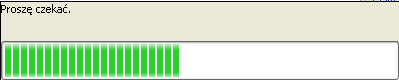
\includegraphics[width=0.45\textwidth]{images/netwrokScanningW}}    
  \hspace{1mm}
  \subfloat[Linux]{
\includegraphics[width=0.45\textwidth]{images/netwrokScanningL}}
\caption{Skanowanie sieci} 	
\label{netwrokScanning}
\end{figure}

\begin{figure}[!htb]
\centering 		
  \subfloat[Windows]{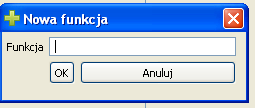
\includegraphics[width=0.35\textwidth]{images/newFunctionW}}    
  \hspace{1mm}
  \subfloat[Linux]{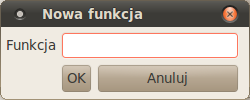
\includegraphics[width=0.35\textwidth]{images/newFunctionL}}
\caption{Okno dodawania funkcji} 	
\label{newFunction}
\end{figure}

\begin{figure}[!htb]
\centering 		
  \subfloat[Windows]{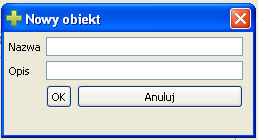
\includegraphics[width=0.35\textwidth]{images/newObjectW}}    
  \hspace{1mm}
  \subfloat[Linux]{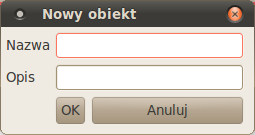
\includegraphics[width=0.35\textwidth]{images/newObjectL}}
\caption{Okno dodawania obiektu} 	
\label{newObject}
\end{figure}

\begin{figure}[!htb]
\centering 		
  \subfloat[Windows]{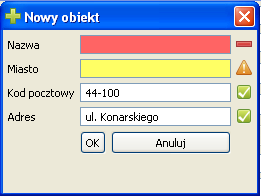
\includegraphics[width=0.35\textwidth]{images/newPlaceErrorW}}    
  \hspace{1mm}
  \subfloat[Linux]{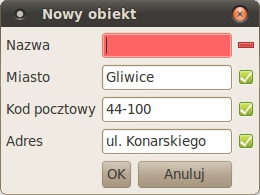
\includegraphics[width=0.35\textwidth]{images/newPlaceErrorL}}
\caption{Błąd przy dodawaniu nowego miejsca} 	
\label{newPlaceError}
\end{figure}

\begin{figure}[!htb]
\centering 		
  \subfloat[Windows]{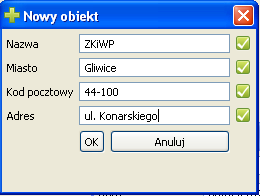
\includegraphics[width=0.35\textwidth]{images/newPlaceW}}    
  \hspace{1mm}
  \subfloat[Linux]{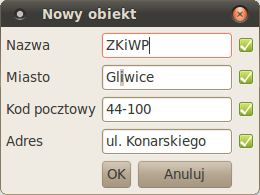
\includegraphics[width=0.35\textwidth]{images/newPlaceL}}
\caption{Okno dodawania miejsca} 	
\label{newPlace}
\end{figure}

\begin{figure}[!htb]
\centering 		
  \subfloat[Windows]{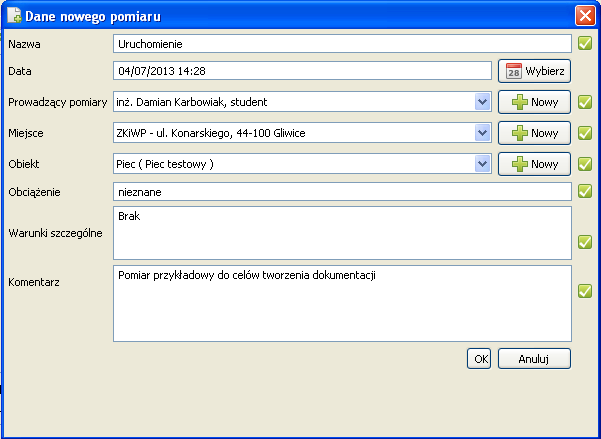
\includegraphics[width=0.49\textwidth]{images/newSurveyFilledW}}    
  \hspace{1mm}
  \subfloat[Linux]{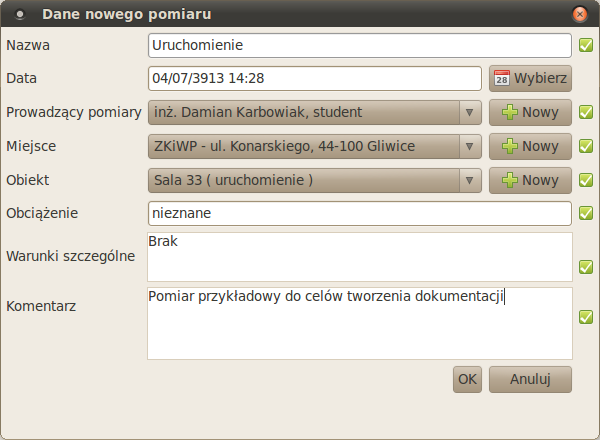
\includegraphics[width=0.49\textwidth]{images/newSurveyFilledL}}
\caption{Okno dodawania pomiaru po prawidłowym wypełnieniu} 	
\label{newSurveyFilled}
\end{figure}

\begin{figure}[!htb]
\centering 		
  \subfloat[Windows]{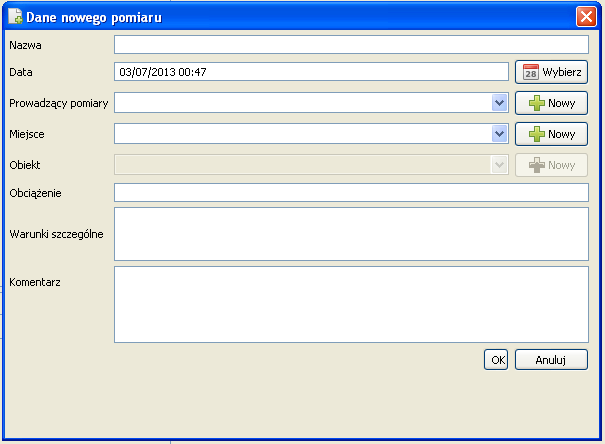
\includegraphics[width=0.45\textwidth]{images/newSurveyW}}    
  \hspace{1mm}
  \subfloat[Linux]{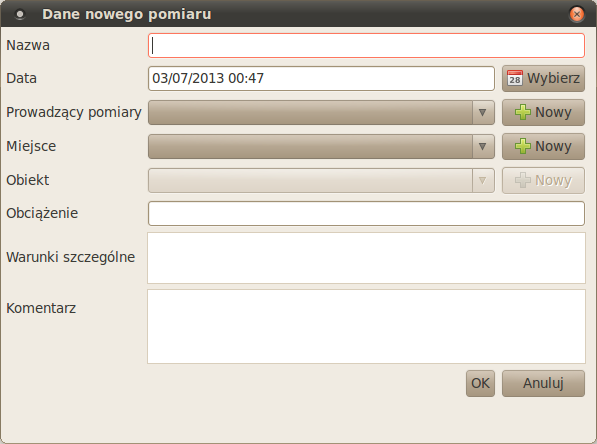
\includegraphics[width=0.45\textwidth]{images/newSurveyL}}
\caption{Okno dodawania pomiaru} 	
\label{newSurvey}
\end{figure}

\begin{figure}[!htb]
\centering 		
  \subfloat[Windows]{\includegraphics[width=0.35\textwidth]{images/newTitleW}}    
  \hspace{1mm}
  \subfloat[Linux]{\includegraphics[width=0.35\textwidth]{images/newTitleL}}
\caption{Okno dodawania tytułu naukowego} 	
\label{newTitle}
\end{figure}

\begin{figure}[!htb]
\centering 		
  \subfloat[Windows]{\includegraphics[width=0.35\textwidth]{images/newUserW}}    
  \hspace{1mm}
  \subfloat[Linux]{\includegraphics[width=0.35\textwidth]{images/newUserL}}
\caption{Okno dodawania użytkownika} 	
\label{newUser}
\end{figure}

\begin{figure}[!htb]
\centering 		
  \subfloat[Windows]{\includegraphics[width=0.49\textwidth]{images/openSurveyW}}    
  \hspace{1mm}
  \subfloat[Linux]{\includegraphics[width=0.49\textwidth]{images/openSurveyL}}
\caption{Okno otwierania pomiaru} 	
\label{openSurvey}
\end{figure}

\begin{figure}[!htb]
\centering 		
  \subfloat[Windows]{\includegraphics[width=0.45\textwidth]{images/reportPDFW}}    
  \hspace{1mm}
  \subfloat[Linux]{\includegraphics[width=0.45\textwidth]{images/reportPDFL}}
\caption{Okno generowania raportu PDF} 	
\label{reportPDF}
\end{figure}

\begin{figure}[!htb]
\centering 		
  \subfloat[Windows]{\includegraphics[width=0.45\textwidth]{images/reportXLSW}}    
  \hspace{1mm}
  \subfloat[Linux]{\includegraphics[width=0.45\textwidth]{images/reportXLSL}}
\caption{Okno generowania raportu XLS} 	
\label{reportXLS}
\end{figure}

\begin{figure}[!htb]
\centering 		
  \subfloat[Windows]{\includegraphics[width=0.45\textwidth]{images/rxtxErrorW}}    
  \hspace{1mm}
  \subfloat[Linux]{\includegraphics[width=0.45\textwidth]{images/rxtxErrorL}}
\caption{Okno błędu braku biblioteki RXTX} 	
\label{rxtxError}
\end{figure}

\begin{figure}[!htb]
\centering 		
  \subfloat[Windows]{\includegraphics[width=0.45\textwidth]{images/splashScreenW}}    
  \hspace{1mm}
  \subfloat[Linux]{\includegraphics[width=0.45\textwidth]{images/splashScreenL}}
\caption{Okno ładowania aplikacji} 	
\label{splashScreen}
\end{figure}

\begin{figure}[!htb]
\centering 		
  \subfloat[Windows]{\includegraphics[width=0.45\textwidth]{images/suggestionW}}    
  \hspace{1mm}
  \subfloat[Linux]{\includegraphics[width=0.45\textwidth]{images/suggestionL}}
\caption{Okno wysyłanie sugestii poprzez email} 	
\label{suggestion}
\end{figure}

Test ikon na Rysunku~\ref{icons:add}
\begin{figure}[!htb]
\centering
\begin{tabular}{ccccc}
\subfloat[Aplikacja]{\makebox[.2\textwidth]{\begin{tabular}{l} \includegraphics{images/application}\label{icons:application} \end{tabular}}} &  
\subfloat[Nowy pomiar]{\makebox[.2\textwidth]{\begin{tabular}{l} \includegraphics{images/newSurvey}\label{icons:newSurvey} \end{tabular}}} &  
\subfloat[Otwórz pomiar]{\makebox[.2\textwidth]{\begin{tabular}{l} \includegraphics{images/dir}\label{icons:dir} \end{tabular}}} &
\subfloat[Wyłącz program]{\makebox[.2\textwidth]{\begin{tabular}{l} \includegraphics{images/shutdown}\label{icons:shutdown} \end{tabular}}} &
\subfloat[Odśwież]{\makebox[.2\textwidth]{\begin{tabular}{l} \includegraphics{images/odswiez}\label{icons:odswiez} \end{tabular}}} \\

\subfloat[PDF]{\makebox[.2\textwidth]{\begin{tabular}{l} \includegraphics{images/pdfIco}\label{icons:pdfIco} \end{tabular}}} &
\subfloat[XLS]{\makebox[.2\textwidth]{\begin{tabular}{l} \includegraphics{images/excel}\label{icons:excel} \end{tabular}}} &
\subfloat[Ok]{\makebox[.2\textwidth]{\begin{tabular}{l} \includegraphics{images/ok}\label{icons:ok} \end{tabular}}} &  
\subfloat[Ostrzeżenie]{\makebox[.2\textwidth]{\begin{tabular}{l} \includegraphics{images/warning}\label{icons:warning} \end{tabular}}} &
\subfloat[Błąd]{\makebox[.2\textwidth]{\begin{tabular}{l} \includegraphics{images/error}\label{icons:error} \end{tabular}}} \\

\subfloat[Dodawanie]{\makebox[.2\textwidth]{\begin{tabular}{l} \includegraphics{images/add}\label{icons:add} \end{tabular}}} &  
\subfloat[Edytuj]{\makebox[.2\textwidth]{\begin{tabular}{l} \includegraphics{images/edit}\label{icons:edit} \end{tabular}}} &  
\subfloat[Kalendarz]{\makebox[.2\textwidth]{\begin{tabular}{l} \includegraphics{images/calendar}\label{icons:calendar} \end{tabular}}} &  
\subfloat[Użytkownik]{\makebox[.2\textwidth]{\begin{tabular}{l} \includegraphics{images/user}\label{icons:user} \end{tabular}}} &  
\subfloat[Anuluj]{\makebox[.2\textwidth]{\begin{tabular}{l} \includegraphics{images/cancel}\label{icons:cancel} \end{tabular}}} \\

\subfloat[Preferencje]{\makebox[.2\textwidth]{\begin{tabular}{l} \includegraphics{images/preferences}\label{icons:preferences} \end{tabular}}} &  
\subfloat[Pomoc]{\makebox[.2\textwidth]{\begin{tabular}{l} \includegraphics{images/help}\label{icons:help} \end{tabular}}} &
\subfloat[O programie]{\makebox[.2\textwidth]{\begin{tabular}{l} \includegraphics{images/about}\label{icons:about} \end{tabular}}} &  
\subfloat[Mail]{\makebox[.2\textwidth]{\begin{tabular}{l} \includegraphics{images/mail}\label{icons:mail} \end{tabular}}} &  
\subfloat[Wysyłanie maila]{\makebox[.2\textwidth]{\begin{tabular}{l} \includegraphics{images/mail_send}\label{icons:mail_send} \end{tabular}}} \\

\subfloat[Połącz]{\makebox[.2\textwidth]{\begin{tabular}{l} \includegraphics{images/connect}\label{icons:connect} \end{tabular}}} &  
\subfloat[Rozłącz]{\makebox[.2\textwidth]{\begin{tabular}{l} \includegraphics{images/disconnect}\label{icons:disconnect} \end{tabular}}} &  
\subfloat[Start]{\makebox[.2\textwidth]{\begin{tabular}{l} \includegraphics{images/run}\label{icons:run} \end{tabular}}} &
\subfloat[Stop]{\makebox[.2\textwidth]{\begin{tabular}{l} \includegraphics{images/stop}\label{icons:stop} \end{tabular}}} &  
\subfloat[Komentarz]{\makebox[.2\textwidth]{\begin{tabular}{l} \includegraphics{images/comment}\label{icons:comment} \end{tabular}}} \\
\end{tabular}  		
\caption{Ikony wykorzystywane w aplikacji} 	
\label{icons}
\end{figure}

\begin{figure}[!htb] 	\centering 	\includegraphics[width=0.99\textwidth]{images/pdf} 	\caption{Przykładowy raport PDF} \label{reportPDFfinal} \end{figure} 

\begin{figure}[!htb] 	\centering 	\includegraphics[width=0.99\textwidth]{images/xls} 	\caption{Przykładowy raport XLS} \label{reportXLSfinal} \end{figure} 


\end{document}